\chapter{Antimicrobial resistance}

\section{Antimicrobial resistance disaster}

People discovered antimicrobials in order to destroy microbes which cause diseases and harm the health. The most popular antimicrobials are antibiotics that fight bacteria. Other types of antimicrobials are anti-parasites, antifungals (from fungi) and antivirals (from viruses). Penicillin, the first commercialized antibiotic, was discovered in 1928 by Alexander Fleming [3].  Until 1945, it wasn’t used and distributed. However, during the World War II, every surgical operation and medical cure was accompanied with penicillin. At that time, it was like a “miracle drug” and people thought that they won the infections which would not be seen in the future.  But when Fleming won the Nobel Prize for penicillin, he warned of bacteria becoming resistant to penicillin in his acceptance speech [3].

\begin{figure}[H]
  \centering
  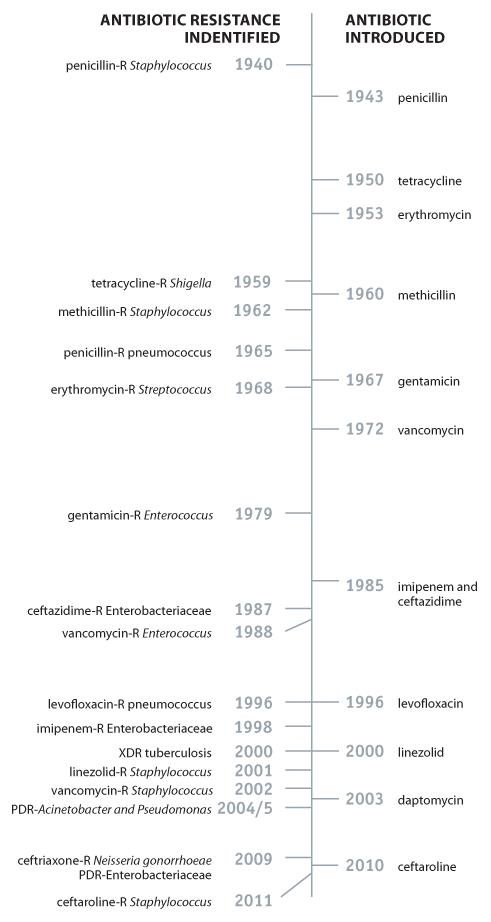
\includegraphics[width=0.5\textwidth]{img/Fig1}
  \caption{History of Antibiotics}
  \label{fig1}
\end{figure}

As it can be seen in Figure 1, discovery of new antibiotics always involved antibiotic resistance. When antimicrobial resistance was found, people started to search for new antibiotics and cure the AMR with the other similar drugs. And further, the use of antibiotics started to increase worldwide. Today, people can buy antibiotics without doctor’s prescription in any shop and drugstore in order not to waste time. Also, some people just take the antibiotics without any reason believing that they will prevent some diseases and infections. Therefore, nowadays, the consumption of antibiotics exceeded the accepted norm (see Figure 2) [4]. According to Health Report of the Organization for Economic Co-operation and Development (OECD), there is a huge overuse and misuse of antibiotics in such countries as Turkey, Greece and France [4]. The chart below describes the daily dose of antibiotic per 1000 population used per one day. And this is one of the reasons for antibiotic resistance because it’s assumed that more antibiotics lead to the increase of the probability that antibiotic resistance occurs.

\begin{figure}[H]
  \centering
  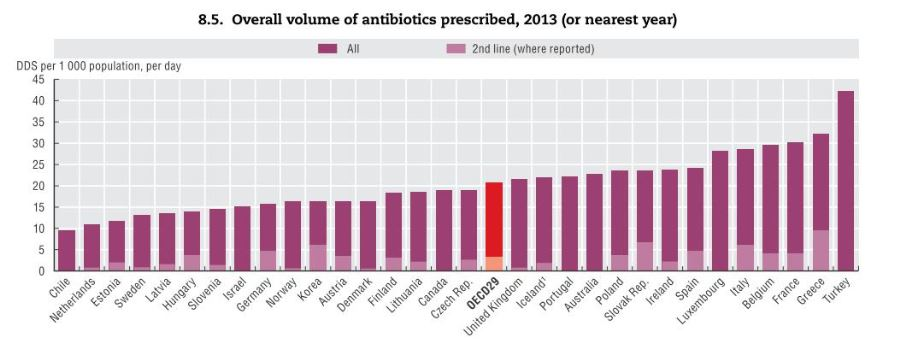
\includegraphics[width=0.8\textwidth]{img/Fig2}
  \caption{Overall volume of prescribed antibiotics by country}
  \label{fig2}
\end{figure}

So, antimicrobial resistance is an increasing problem among the whole humanity. A solution for it still has not been discovered yet, therefore the optimal usage of the antibiotics is very important for our population. Antibiotics are very special type of medicine, which is used against bacterial diseases and often can be considered as the only possible treatment for a patient. The chemical structure of antibiotics let them effectively devastate exponentially growing populations of bacteria. In order to treat a disease effectively, doctors prescribe a specific antibiotic with specific course of usage. The antibiotics are usually needed to be used in specific doses within specific periods of time. The exact timing of treatment and accurate dosing of the medicine is very important for the right effect of the antibiotic. However, people usually lack the information about antibiotics and start to cure themselves by own methods. When patients do not follow the prescribed conditions and rules of antibiotic usage or the doctors were mistaken to give the wrong antibiotic, they allow the bacteria to develop immunity against the antibiotic medicine (see Figure 2) [3]. This is in fact an amazing biological property, which shows how living creatures are able to adapt to different murderous enemies and conditions.

\begin{figure}[H]
  \centering
  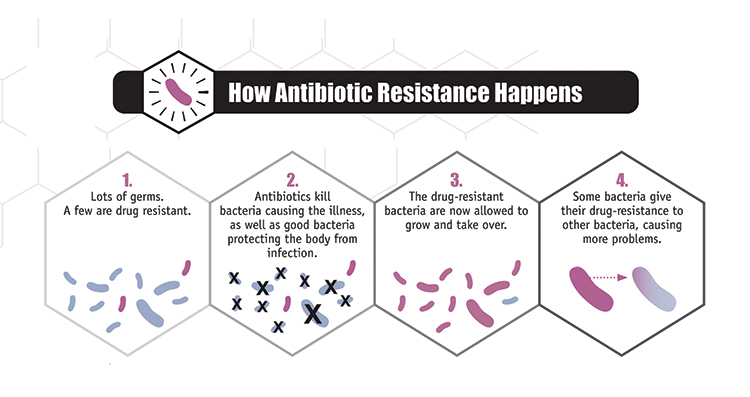
\includegraphics[width=0.8\textwidth]{img/Fig3}
  \caption{How Antibiotic Resistance happens}
  \label{fig3}
\end{figure}

One of the main reasons why antibiotics lose their effectiveness lies behind the failure to appropriately conduct the treatment course with an antibiotic. The schedule of antibiotic usage during the treatment course has been accurately developed by pharmaceutical specialists. The course is usually designed so that the population of bacteria is effectively reduced with the medicine. The doses of the antibiotic are not too much to potentially harm the patient’s organism and are not too little to result in adaption of the bacteria. Adhering to the doctor’s prescriptions in terms of timing and dosing is crucial for an effective and successful treatment of a disease. Individuals that do not follow these rules and violate the prescription conditions are not only making their own treatment ineffective and even dangerous. They are also responsible for the process of antibiotic resistance. By exposing bacteria to insufficient amounts of the antibiotic, a patient stimulates the natural ability of the organisms to develop some immunity mechanisms against the killing medicine. This way, irresponsible patients are strengthening different dangerous microorganisms and reducing the power of the weapons that are used to fight against them.

Another major problem with the protection of antibiotics is related to wrong prescriptions. In many countries, where the level of education is not as high as necessary, there are many unqualified or low-qualification medical workers. This is not only a property of developing countries, but also may appear in more developed societies, too. There are doctors who prescribe antibiotics without knowing the real reason behind the disease. In this case, the antibiotics are useless, and only get exposed to the internal micro-flora of the patient, making unpredictable changes on the bacterial level. There may occur cases when patients really need antibiotics; however doctors prescribe a wrong one. Though this may accidentally lead to treatment, the bacteria, which get exposed to the antibiotic, may start becoming resistant to that medicine. Finally, there are cases when doctors prescribe wrong doses and wrong periods of antibiotic treatment course. This is also a very probable opportunity for a bacterial population to get resistant by confronting small doses of the antibiotic.

\section{Antibiotics Abuse}

Recently, there has been a tendency among people related to farming to use antibiotics as nutrition for animals. The feeding of animals with antibiotics tends to result in larger body sizes, meaning more meat for production. Many farmers are feeding animals like cows, horses, pigs, and chicken with antibiotics and are getting fatter livestock and correspondingly larger amounts of produced meat. Eventually, this meat is eaten by consumers, i.e. by ordinary people, who in turn receive those antibiotics with the meat. This way, antibiotics can reach our organisms through the animal food that we consume as in can be seen in Figure 3 [3]. Since this kind of antibiotic "use" is not at all controlled by medical specialists, the bacteria inside our bodies again have a great opportunity to evolve and become stronger against specific chemicals. As a result, the usage of antibiotics in farming is a very destructive and seamless way of antibiotic resistance development.

\begin{figure}[H]
  \centering
  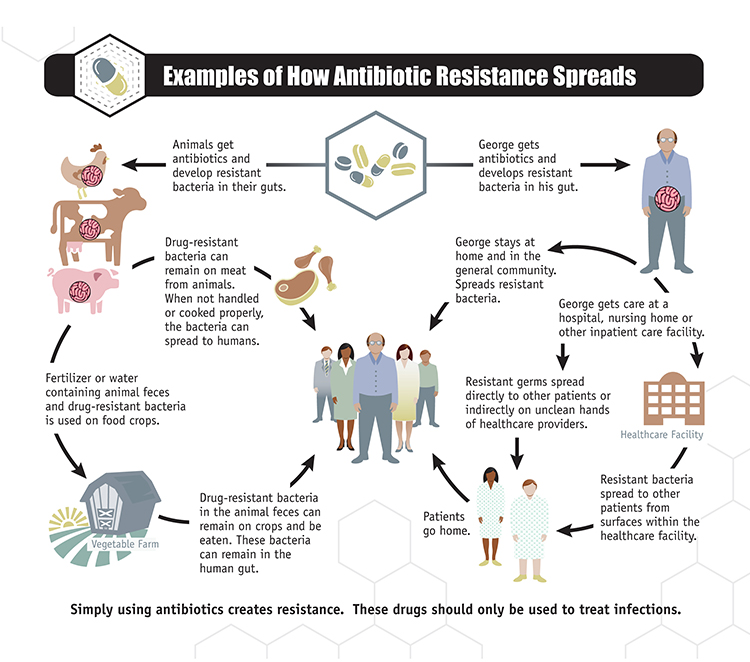
\includegraphics[width=0.8\textwidth]{img/Fig4}
  \caption{How Antibiotic Resistance spreads}
  \label{fig4}
\end{figure}

As we can see, the effectiveness of existing antibiotics is rapidly decreasing as their abuse is continued to be done in different ways. The humanity could probably continue to abuse them this way, provided that the discovery of new antibiotics is being made at a sufficient rate. However, the situation in new antibiotics discovery is even worse. There hasn't been any new antibiotic discoveries since late 1980-s. This is a huge gap in research and development of antibiotics. One of the most recent discovered antibiotics is teixobactin, which is dated to January 2016. Creation of new antibiotics is a very long and difficult process that includes multiple laboratory experiments, in chemical tubes as well as on living organisms. So, it took over 30 years to discover new antibiotic (see Figure 4). In the light of this difficulty, it is very ineffective that people are losing the effectiveness of their only weapons against killing bacteria.

\begin{figure}[H]
  \centering
  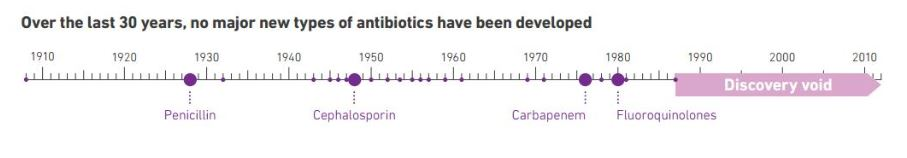
\includegraphics[width=\textwidth]{img/Fig5}
  \caption{Discovery of new antibiotics}
  \label{fig5}
\end{figure}

If we look at the current statistics, cases of antibiotic resistance are increasing for such dangerous diseases as Tuberculosis, HIV, Malaria, Influenza, etc. The most dangerous contagious disease that can cause fatal consequences and whose behavior is difficult to predict is Influenza. Seasonal influenza is an acute viral infection caused by an influenza virus. There are three types of seasonal influenza – A, B and C. Type A influenza viruses are further typed into subtypes according to different kinds and combinations of virus surface proteins. Among many subtypes of influenza A viruses, currently influenza A (H1N1) and A(H3N2) subtypes are circulating among humans. Influenza viruses circulate in every part of the world. Type C influenza cases occur much less frequently than A and B. That is why only influenza A and B viruses are included in seasonal influenza vaccines. Seasonal influenza is characterized by a sudden onset of high fever, cough (usually dry), headache, muscle and joint pain, severe malaise (feeling unwell), sore throat and runny nose. Most people recover from fever and other symptoms within a week without requiring medical attention. But influenza can cause severe illness or death in elder people and children. The time from infection to illness, known as the incubation period, is about two days. Influenza worldwide produces 3–5 million severe illnesses annually and kills an estimated 250,000–500,000 people. [1] Once the flu outbreaks, it creates the epidemic and it’s hard to control its spread and prevent the morbidity and mortality. Moreover, there is a possibility each year that seasonal flu epidemic can give rise to so-called influenza pandemic. An influenza pandemic is an epidemic of an influenza virus that spreads on a worldwide scale and infects a large proportion of the human population.[2]

Influenza pandemics occur when a new strain of the influenza virus is transmitted to humans from another animal species mostly pigs, chickens and ducks. So, the flu virus mutates and new form of the flu is generated which cannot be treated neither by the human immunity nor by vaccinations as it’s completely novel and unknown disease. Thus, such flu spreads extremely rapidly and infects very large numbers of people. In contrast to the regular seasonal epidemics of influenza, these pandemics occur irregularly, with the 1918 Spanish flu the most serious pandemic in recent history. Pandemics can cause high levels of mortality, with the 1918 Spanish influenza pandemic estimated as being responsible for the deaths of approximately 50 million people or more. There have been about three influenza pandemics in each century for the last 300 years. The most recent one was the 2009 flu pandemic. In order to be ready for any outcome and prevent the deaths, health care segment must react as quickly as possible not to let the disease spread to other regions and kill lives. Furthermore, the flu epidemics occur mostly in Asian developing countries where there are poor living conditions and thus, there is a high risk that it can transform to pandemic. And as it’s known, Kazakhstan is located near those susceptible countries like China, Malaysia and can be one of the first infected regions. So, preventive measures would be a key solution to flu tracking.

For example, let’s take Tuberculosis disease. It’s the most “killing” infectious disease in the world which occurs mostly in developing countries with poor conditions and low income. Also, its cure lasts for a very long time and then becoming chronic. People actually don’t fully recover from tuberculosis because their immunity system will be very weak and sensitive to other diseases. Its increasing prevalence in the world caused anti-TB drug resistance increase respectively (see Figure 6). Besides, it is very common in Kazakhstan and spread all over the country as most people used to ignore the disease and avoid hospitals.

\begin{figure}[H]
  \centering
  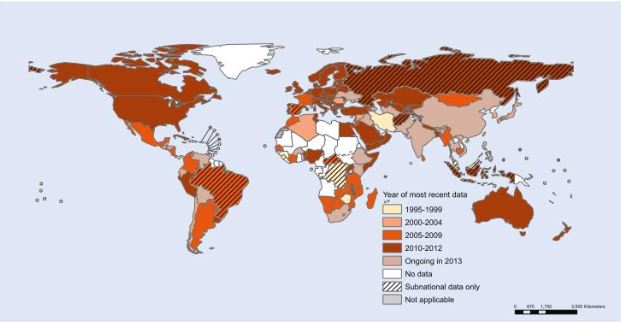
\includegraphics[width=0.8\textwidth]{img/Fig6}
  \caption{Global coverage of anti-TB drug resistance, 1994-2012}
  \label{fig6}
\end{figure}

Another trend seen in Figure 7 proves that tuberculosis is becoming drug resistant from year to year. With this trend, there is likelihood that tuberculosis will become incurable in the future.

\begin{figure}[H]
  \centering
  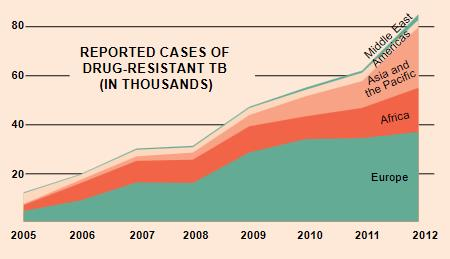
\includegraphics[width=0.7\textwidth]{img/Fig7}
  \caption{Drug resistant tuberculosis by year}
  \label{fig7}
\end{figure}

Tuberculosis can be not only drug resistant, but also multidrug resistant (MDR) and extensively drug resistant (XDR). MDR means that there are bacteria which do not react to 2 most strong anti-TB drugs (rifampisin and isoniazid) [4]. And XDR means that bacteria are resistant to at least 4 anti-TB drugs. It’s the most harmful form of disease which requires long time to cure. Specifically tuberculosis is very dangerous for Kazakhstan because according to World Health Organization’s global report on antimicrobial resistance in 2014, our country is among the regions that have the highest proportions of MDR-TB patients (see Figure 8).

\begin{figure}[H]
  \centering
  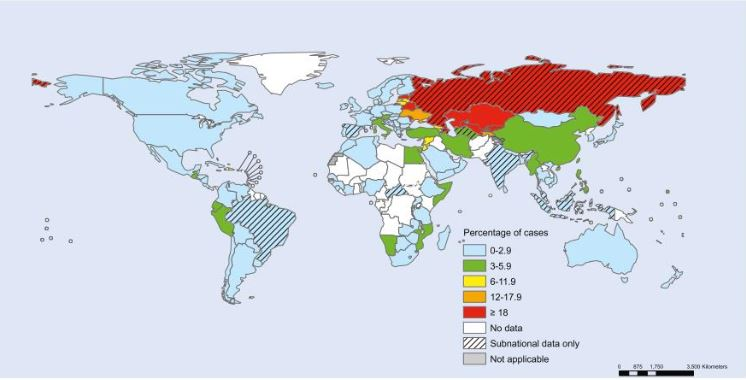
\includegraphics[width=0.8\textwidth]{img/Fig8}
  \caption{Proportion of new TB cases with multidrug resistance (MDR-TB) worldwide}
  \label{fig8}
\end{figure}

Proportions varied up to 35\% and were the highest in Belarus (34,8% in 2012), Kyrgyzstan (26,4% in 2012), Russia (23,1 % in 2011) and Kazakhstan (22,9 % in 2012).

Based on the statistics about antimicrobial resistance and the current situation, World Health Organization forecasts that in the future the majority of deaths will be caused by AMR (see Figure 9).

\begin{figure}[H]
  \centering
  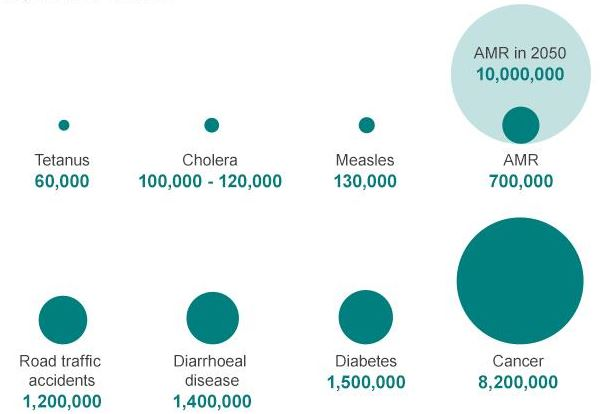
\includegraphics[width=0.7\textwidth]{img/Fig9}
  \caption{Deaths caused by AMR every year compared to other causes of death}
  \label{fig9}
\end{figure}

So, by 2050 people will die mostly due to AMR, not cancer. And the majority of deaths from AMR will specifically occur in Asia by year 2050 as it can be seen in Figure 10.

\begin{figure}[H]
  \centering
  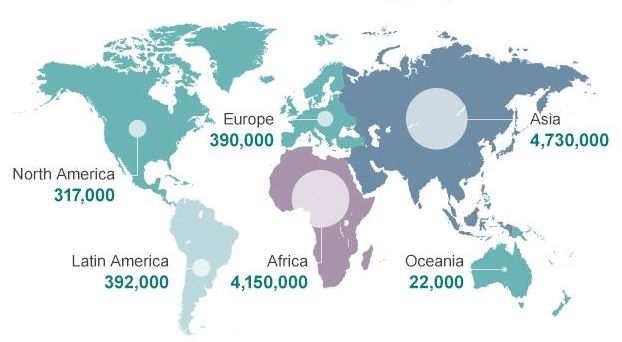
\includegraphics[width=0.9\textwidth]{img/Fig10}
  \caption{Deaths caused by AMR every year by geographical regions by 2050}
  \label{fig10}
\end{figure}

In addition, we shouldn’t ignore the food content. Animals and plants used for our food also consist of antibiotics. According to National Antimicrobial Resistance Monitoring System in United Nations Environment Program (UNEP), resistant bacteria are seen in all types of meat. As it can be seen in Figure 11, the most percentage of antimicrobial resistance appears in chicken.

\begin{figure}[H]
  \centering
  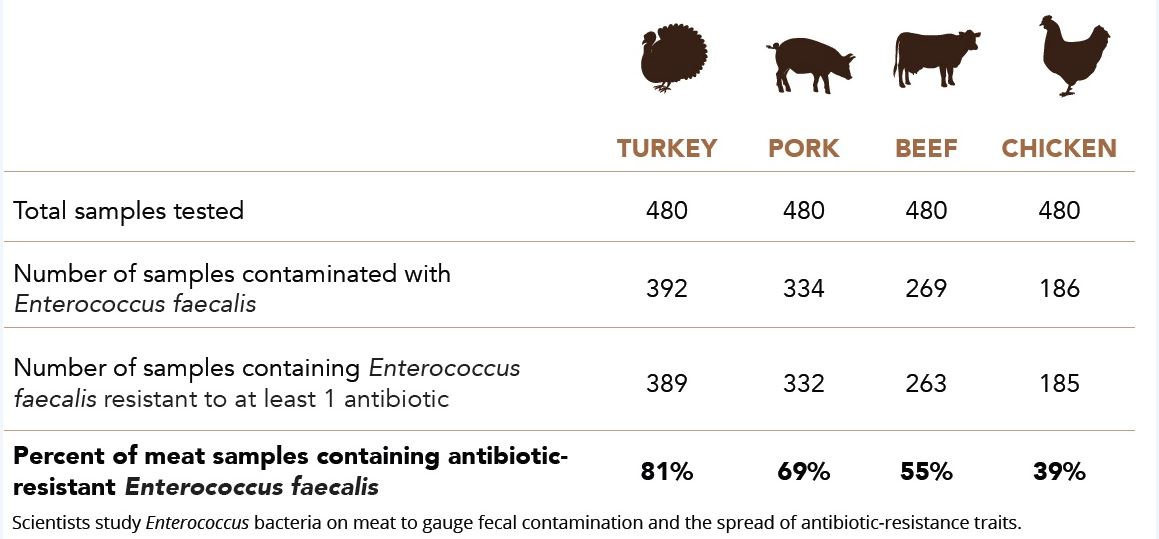
\includegraphics[width=0.8\textwidth]{img/Fig11}
  \caption{Meat samples with resistant bacteria, 2013}
  \label{fig11}
\end{figure}

Also, there is an interesting fact that more antibiotics are used in food animals rather than by humans (see Figure 12).

\begin{figure}[H]
  \centering
  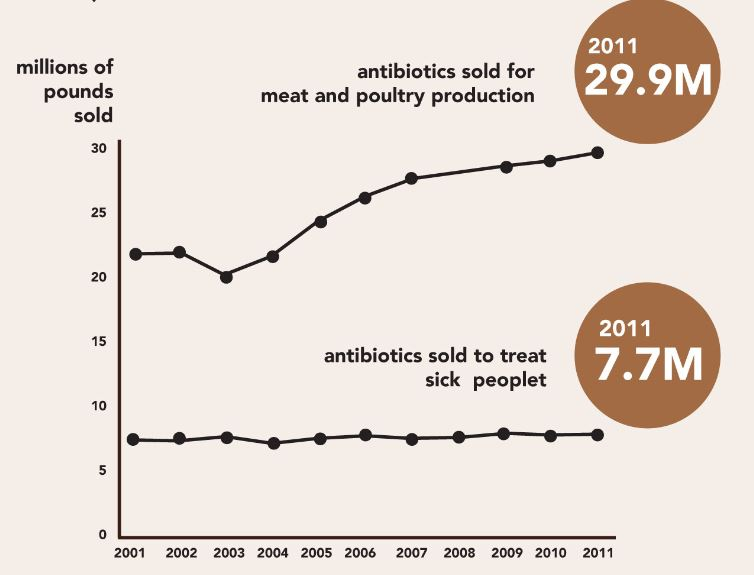
\includegraphics[width=0.8\textwidth]{img/Fig12}
  \caption{Antibiotic sales for meat production and people use}
  \label{fig12}
\end{figure}

So, even people do not use antibiotics, they get them from the meat they eat. And it seems like we would better not eat turkey. We should also check the meat carefully and cook it carefully, buying it from the certified stores.

The most effective way to prevent the disease or severe outcomes from the illness is vaccination. Safe and effective vaccines have been available and used for more than 60 years. Among healthy adults, influenza vaccine can prevent 70\% to 90\% of influenza-specific illness. Among the elderly, the vaccine reduces severe illnesses and complications by up to 60\% and deaths by 80\%. Vaccination is especially important for people at higher risk of serious influenza complications, and for people who live with or care for high risk individuals.

However the vaccination process needs to be carefully considered and optimally planned. Furthermore, vaccination does not always solve the problem. What if new form of disease occurs? When the new flu outbreak happens, immediate measures and actions must be taken in order to prevent deaths.

The prevention of antibiotic / antimicrobial resistance is a global process. This can’t be done by a single person or organization, but rather by the collaboration of many institutions and organizations of the world. It is important to understand, how can we and should we handle this global problem and find a solution for the better future. There are many complexities involved in antimicrobial resistance. Different bacteria may be resistant or susceptible to different types of antibiotics can infect various human populations and etc. In order to understand the problem better, we are considering the mathematical model behind this complex process. The mathematical model can be used to predict ongoing changes in the process as well as understand the key variables involved in the process. Mathematical models can be computed using computer simulations, in order to produce more detailed outcomes.


